% Research Note of the AAS version of main.tex (limits: 1,500 words including title, headers,
% captions and references; 150-word abstract; one figure). Numbers as in main.tex;
% src/check_paper.py checks the limits and headline numbers.

\documentclass[RNAAS]{aastex631}

\graphicspath{{figures/}}

\begin{document}

\title{The Fate of a Hypothetical Second Moon of Earth}

\author{John Rey Ishiguro Quizon}
\affiliation{STI College Legazpi, Legazpi City, Albay, Philippines}

\begin{abstract}
I simulate 12,000 hypothetical second moons of Earth, of $10^{-3}$ to 1 lunar masses at 0.1 to 3
lunar distances on prograde and retrograde orbits, together with the real Sun, Earth and Moon (JPL
Horizons, DE440), for up to 100 years. Overall, 38.0\% survive, 32.0\% are ejected and 27.4\%
collide with Earth. Survivors are concentrated on close orbits near the ecliptic plane; near-polar
orbits are driven into Earth, consistent with Lidov--Kozai cycles, and beyond the Moon's orbit
nearly all survivors are retrograde. Displacing a second moon by 1~m changes about 8\% of
outcomes. A Random Forest trained on the initial orbital elements predicts the outcome of 2,400
held-out systems, evaluated once under criteria fixed in advance, with 85.1\% accuracy (macro-F1
0.711), exceeding a two-variable physics rule (78.9\%), and is about 80,000 times faster than
direct integration in batches.
\end{abstract}

\keywords{Natural satellite dynamics (2212) --- Earth-moon system (436) --- Astronomical
simulations (1857)}

\section{Introduction}

Earth has one large satellite, but a second, smaller moon may once have existed:
\citet{Jutzi2011} proposed that the lunar farside highlands formed when a companion moon collided
with the Moon. Simulations of packed moon systems around an Earth-mass planet find that only a few
Moon-mass satellites can coexist \citep{Satyal2022}, and solar tides limit stable satellite orbits
to a fraction of the planet's Hill radius, farther out for retrograde orbits \citep{Domingos2006}.
Here I map the fate of a single additional moon of the present Earth--Moon system and test whether
a machine-learning surrogate, in the spirit of \citet{Tamayo2020}, can predict it without
integration.

\section{Methods}

I integrate the Sun, Earth, Moon and a second moon with REBOUND and its IAS15 integrator
\citep{Rein2012, Rein2015}, starting from JPL Horizons states at 2026-01-01 TDB \citep[DE440;][]{Park2021}.
Without a second moon, the simulated Moon stays within 10.3~km of the ephemeris over one year.
Second moons have the Moon's density. Mass and semi-major axis are drawn log-uniformly, and
eccentricity (0--0.8), inclination (0--180$^\circ$) and the orientation angles uniformly; orbits
with periapsis inside the Roche limit are redrawn. Each system runs for up to 100 years and ends at
the first collision or ejection. Before any analysis, 2,400 systems (20\%, stratified by outcome)
were held out.

The surrogate predicts four classes (survived, ejected, collided with Earth, and Moon interaction:
a collision with or loss of the Moon) from the orbital elements and derived quantities such as
periapsis, apoapsis and $|\cos i|$. Inputs, model and hyperparameters were chosen by
cross-validation on the 9,600 training systems, with nested tuning; a Random Forest
\citep{Breiman2001, Pedregosa2011} performed best. Its criteria for the single test evaluation
(macro-F1 within the cross-validated 95\% interval, 0.708--0.737; a gain over a depth-3 decision
tree on apoapsis and $|\cos i|$; calibrated survival probabilities) were recorded before the test
set was opened. To measure chaos, 1,500 training systems were integrated again with the second
moon displaced by 1~m.

\section{Results}

Of the 12,000 second moons, 38.0\% survive 100 years, 32.0\% are ejected, 27.4\% collide with
Earth and 1.4\% with the Moon; in 1.2\% of systems the Moon is lost. Figure~\ref{fig:rnaas}a shows
where survivors lie. Inside 0.5 lunar distances, 96.5\% of orbits with inclinations below
45$^\circ$ or above 135$^\circ$ survive, whereas 99.1\% of near-polar orbits collide with Earth,
consistent with Lidov--Kozai cycles \citep{Kozai1962, Lidov1962}. Orbits that cross the Moon's are
destabilized (3.0\% survive), and survival falls below 10\% at 0.22 Hill radii for both orbit
directions, so the Moon rather than the Sun sets the outer limit. Beyond the Moon's orbit, 11.4\% of
retrograde systems survive against 0.3\% of prograde ones. Survival is not permanent: of 500
survivors integrated to 1,000 years, 21.4\% were lost.

A 1~m displacement changes 7.7\% of outcomes, mostly near the Moon's orbit. On the held-out systems
the Random Forest reaches 85.1\% accuracy and a macro-F1 of 0.711, matching cross-validation
(Figure~\ref{fig:rnaas}b) and exceeding the physics rule (78.9\%, macro-F1 0.591); all criteria
are met, and the survival ROC AUC is 0.988. The model errs on 53.8\% of the test systems whose
outcome changes under a 1~m displacement but on 11.3\% of the others, and the most confident half
of its predictions is 98.2\% correct. Moon interactions remain hard to predict (27\% recall). A
prediction takes 0.11~s alone and 133~$\mu$s per system in a batch, against a median of 2.7~s and a
mean of 10.7~s per integration: 24 times and about 80,000 times faster.

\begin{figure}
\centering
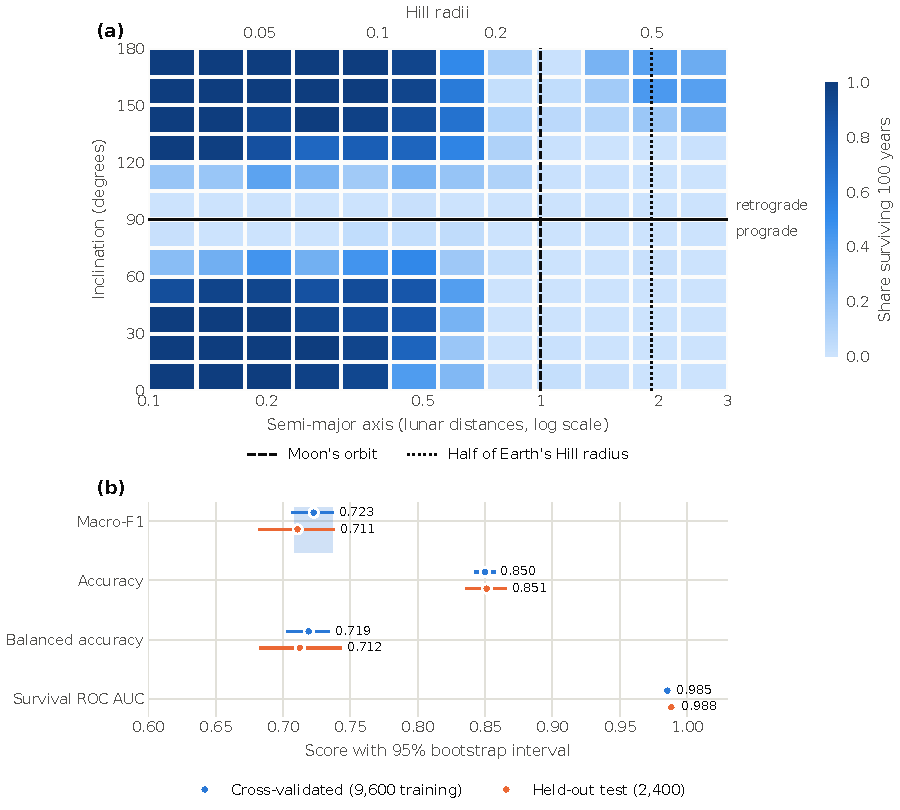
\includegraphics[width=0.92\textwidth]{rnaas_figure.pdf}
\caption{(a) Share of the 9,600 training systems surviving 100 years by initial semi-major axis and
inclination (above 90$^\circ$: retrograde). (b) Random Forest scores from cross-validation (blue)
and on the 2,400 held-out systems (orange), with 95\% bootstrap intervals; shaded: the macro-F1
range fixed in advance. \label{fig:rnaas}}
\end{figure}

\newpage
\section{Discussion}

The fate of a second moon is set mainly by the Moon, through close encounters and, for inclined
orbits, Lidov--Kozai cycles, and depends on two simple quantities: whether the orbit reaches the
Moon's distance and how far its inclination is from 90$^\circ$. Chaos limits any prediction from
initial conditions, and the surrogate's errors concentrate where outcomes are chaotic, so its
confident predictions can replace integrations while uncertain systems near the Moon's orbit are
simulated directly. Outcome shares depend on the sampling design (with isotropic inclinations,
29.7\% survive). The model omits tides, Earth's oblateness and the other planets, and
``survived'' refers to a 100-year horizon.

\section*{Data availability}

Code, configurations, results and a longer account are available at
\url{https://github.com/JreyForFun/two-moons-ml} (MIT license); the dataset is archived on Zenodo
\citep{Quizon2026data}.

\begin{acknowledgments}
This work made use of the JPL Horizons on-line solar system data service. The author used an AI
assistant (Claude, Anthropic) for help with code development and manuscript drafting; all
analyses, results and text were reviewed and verified by the author.
\end{acknowledgments}

\bibliography{references}{}
\bibliographystyle{aasjournal}

\end{document}
